\begin{figure}[h]
    \begin{subfigure}{\linewidth}
      \centering
      $
      \begin{array}{l}
      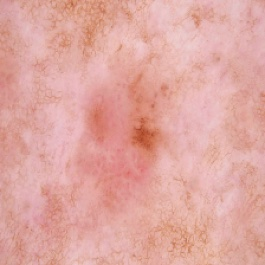
\includegraphics[width=0.26\linewidth]{graphics/ResNet-50/derm_unperturbed.jpg}
      \end{array}
      \mathlarger{\mathlarger{\mathlarger{\mathlarger{+}}}}
      \begin{array}{l}
        
\includegraphics[width=0.26\linewidth]{graphics/ResNet-50/derm_e=0.01_difference.jpg}
      \end{array}
      \mathlarger{\mathlarger{\mathlarger{\mathlarger{=}}}}
      \begin{array}{l}
        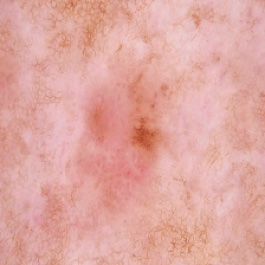
\includegraphics[width=0.26\linewidth]{graphics/ResNet-50/derm_e=0.01.jpg}
      \end{array}
      $
      \caption{An example of $\epsilon=0.01$ perturbation on the dermatoscopy dataset. 0.01 is the maximum perturbation radius used for this dataset.\\}
      \label{example_derm_perturbation}
    \end{subfigure}
    
    \begin{subfigure}{\linewidth}
      \centering
      $
      \begin{array}{l}
      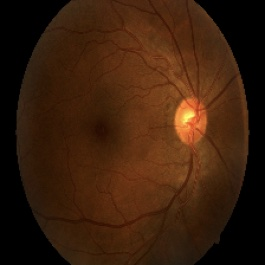
\includegraphics[width=0.26\linewidth]{graphics/ResNet-50/dr_unperturbed.jpg}
      \end{array}
      \mathlarger{\mathlarger{\mathlarger{\mathlarger{+}}}}
      \begin{array}{l}
        
\includegraphics[width=0.26\linewidth]{graphics/ResNet-50/dr_e=0.32_difference.jpg}
      \end{array}
      \mathlarger{\mathlarger{\mathlarger{\mathlarger{=}}}}
      \begin{array}{l}
        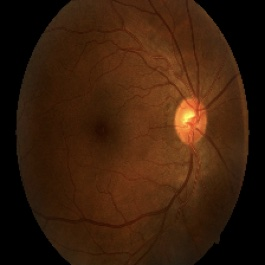
\includegraphics[width=0.26\linewidth]{graphics/ResNet-50/dr_e=0.32.jpg}
      \end{array}
      $
      \caption{An example of $\epsilon=0.32$ perturbation on the fundoscopy dataset. 0.32 is the maximum perturbation radius used for this dataset.\\}
      \label{example_dr_perturbation}
    \end{subfigure}
    \begin{subfigure}{\linewidth}
      \centering
      $
      \begin{array}{l}
      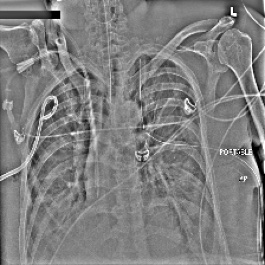
\includegraphics[width=0.26\linewidth]{graphics/ResNet-50/pneumo_unperturbed.jpg}
      \end{array}
      \mathlarger{\mathlarger{\mathlarger{\mathlarger{+}}}}
      \begin{array}{l}
        
\includegraphics[width=0.26\linewidth]{graphics/ResNet-50/pneumo_e=0.32_difference.jpg}
      \end{array}
      \mathlarger{\mathlarger{\mathlarger{\mathlarger{=}}}}
      \begin{array}{l}
        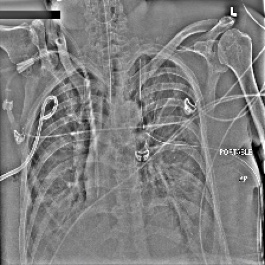
\includegraphics[width=0.26\linewidth]{graphics/ResNet-50/pneumo_e=0.32.jpg}
      \end{array}
      $
      \caption{An example of $\epsilon=0.32$ perturbation on the chest x-ray dataset. 0.32 is the maximum perturbation radius used for this dataset.\\}
      \label{example_pneumo_perturbation}
    \end{subfigure}%
    \caption{Perturbation examples}
  \end{figure}